\documentclass[twoside]{book}

% Packages required by doxygen
\usepackage{fixltx2e}
\usepackage{calc}
\usepackage{doxygen}
\usepackage[export]{adjustbox} % also loads graphicx
\usepackage{graphicx}
\usepackage[utf8]{inputenc}
\usepackage{makeidx}
\usepackage{multicol}
\usepackage{multirow}
\PassOptionsToPackage{warn}{textcomp}
\usepackage{textcomp}
\usepackage[nointegrals]{wasysym}
\usepackage[table]{xcolor}

% Font selection
\usepackage[T1]{fontenc}
\usepackage[scaled=.90]{helvet}
\usepackage{courier}
\usepackage{amssymb}
\usepackage{sectsty}
\renewcommand{\familydefault}{\sfdefault}
\allsectionsfont{%
  \fontseries{bc}\selectfont%
  \color{darkgray}%
}
\renewcommand{\DoxyLabelFont}{%
  \fontseries{bc}\selectfont%
  \color{darkgray}%
}
\newcommand{\+}{\discretionary{\mbox{\scriptsize$\hookleftarrow$}}{}{}}

% Page & text layout
\usepackage{geometry}
\geometry{%
  a4paper,%
  top=2.5cm,%
  bottom=2.5cm,%
  left=2.5cm,%
  right=2.5cm%
}
\tolerance=750
\hfuzz=15pt
\hbadness=750
\setlength{\emergencystretch}{15pt}
\setlength{\parindent}{0cm}
\setlength{\parskip}{3ex plus 2ex minus 2ex}
\makeatletter
\renewcommand{\paragraph}{%
  \@startsection{paragraph}{4}{0ex}{-1.0ex}{1.0ex}{%
    \normalfont\normalsize\bfseries\SS@parafont%
  }%
}
\renewcommand{\subparagraph}{%
  \@startsection{subparagraph}{5}{0ex}{-1.0ex}{1.0ex}{%
    \normalfont\normalsize\bfseries\SS@subparafont%
  }%
}
\makeatother

% Headers & footers
\usepackage{fancyhdr}
\pagestyle{fancyplain}
\fancyhead[LE]{\fancyplain{}{\bfseries\thepage}}
\fancyhead[CE]{\fancyplain{}{}}
\fancyhead[RE]{\fancyplain{}{\bfseries\leftmark}}
\fancyhead[LO]{\fancyplain{}{\bfseries\rightmark}}
\fancyhead[CO]{\fancyplain{}{}}
\fancyhead[RO]{\fancyplain{}{\bfseries\thepage}}
\fancyfoot[LE]{\fancyplain{}{}}
\fancyfoot[CE]{\fancyplain{}{}}
\fancyfoot[RE]{\fancyplain{}{\bfseries\scriptsize Generated by Doxygen }}
\fancyfoot[LO]{\fancyplain{}{\bfseries\scriptsize Generated by Doxygen }}
\fancyfoot[CO]{\fancyplain{}{}}
\fancyfoot[RO]{\fancyplain{}{}}
\renewcommand{\footrulewidth}{0.4pt}
\renewcommand{\chaptermark}[1]{%
  \markboth{#1}{}%
}
\renewcommand{\sectionmark}[1]{%
  \markright{\thesection\ #1}%
}

% Indices & bibliography
\usepackage{natbib}
\usepackage[titles]{tocloft}
\setcounter{tocdepth}{3}
\setcounter{secnumdepth}{5}
\makeindex

% Hyperlinks (required, but should be loaded last)
\usepackage{ifpdf}
\ifpdf
  \usepackage[pdftex,pagebackref=true]{hyperref}
\else
  \usepackage[ps2pdf,pagebackref=true]{hyperref}
\fi
\hypersetup{%
  colorlinks=true,%
  linkcolor=blue,%
  citecolor=blue,%
  unicode%
}

% Custom commands
\newcommand{\clearemptydoublepage}{%
  \newpage{\pagestyle{empty}\cleardoublepage}%
}

\usepackage{caption}
\captionsetup{labelsep=space,justification=centering,font={bf},singlelinecheck=off,skip=4pt,position=top}

%===== C O N T E N T S =====

\begin{document}

% Titlepage & ToC
\hypersetup{pageanchor=false,
             bookmarksnumbered=true,
             pdfencoding=unicode
            }
\pagenumbering{alph}
\begin{titlepage}
\vspace*{7cm}
\begin{center}%
{\Large Toms Engine V2 }\\
\vspace*{1cm}
{\large Generated by Doxygen 1.8.14}\\
\end{center}
\end{titlepage}
\clearemptydoublepage
\pagenumbering{roman}
\tableofcontents
\clearemptydoublepage
\pagenumbering{arabic}
\hypersetup{pageanchor=true}

%--- Begin generated contents ---
\chapter{Namespace Index}
\section{Namespace List}
Here is a list of all namespaces with brief descriptions\+:\begin{DoxyCompactList}
\item\contentsline{section}{\mbox{\hyperlink{namespacetomsengine}{tomsengine}} }{\pageref{namespacetomsengine}}{}
\end{DoxyCompactList}

\chapter{Hierarchical Index}
\section{Class Hierarchy}
This inheritance list is sorted roughly, but not completely, alphabetically\+:\begin{DoxyCompactList}
\item \contentsline{section}{tomsengine\+:\+:Audio}{\pageref{classtomsengine_1_1_audio}}{}
\item \contentsline{section}{tomsengine\+:\+:Audio\+Impl}{\pageref{structtomsengine_1_1_audio_impl}}{}
\item \contentsline{section}{tomsengine\+:\+:Component}{\pageref{classtomsengine_1_1_component}}{}
\begin{DoxyCompactList}
\item \contentsline{section}{tomsengine\+:\+:Mesh\+Renderer}{\pageref{classtomsengine_1_1_mesh_renderer}}{}
\end{DoxyCompactList}
\item \contentsline{section}{tomsengine\+:\+:Core}{\pageref{classtomsengine_1_1_core}}{}
\item \contentsline{section}{tomsengine\+:\+:Entity}{\pageref{classtomsengine_1_1_entity}}{}
\item \contentsline{section}{tomsengine\+:\+:Sampler}{\pageref{structtomsengine_1_1_sampler}}{}
\item \contentsline{section}{tomsengine\+:\+:Shader}{\pageref{classtomsengine_1_1_shader}}{}
\item \contentsline{section}{tomsengine\+:\+:Texture}{\pageref{classtomsengine_1_1_texture}}{}
\item \contentsline{section}{tomsengine\+:\+:Vertex\+Array}{\pageref{classtomsengine_1_1_vertex_array}}{}
\item \contentsline{section}{tomsengine\+:\+:Vertex\+Buffer}{\pageref{classtomsengine_1_1_vertex_buffer}}{}
\end{DoxyCompactList}

\chapter{Class Index}
\section{Class List}
Here are the classes, structs, unions and interfaces with brief descriptions\+:\begin{DoxyCompactList}
\item\contentsline{section}{\mbox{\hyperlink{classtomsengine_1_1_audio}{tomsengine\+::\+Audio}} }{\pageref{classtomsengine_1_1_audio}}{}
\item\contentsline{section}{\mbox{\hyperlink{structtomsengine_1_1_audio_impl}{tomsengine\+::\+Audio\+Impl}} }{\pageref{structtomsengine_1_1_audio_impl}}{}
\item\contentsline{section}{\mbox{\hyperlink{classtomsengine_1_1_component}{tomsengine\+::\+Component}} }{\pageref{classtomsengine_1_1_component}}{}
\item\contentsline{section}{\mbox{\hyperlink{classtomsengine_1_1_core}{tomsengine\+::\+Core}} }{\pageref{classtomsengine_1_1_core}}{}
\item\contentsline{section}{\mbox{\hyperlink{classtomsengine_1_1_entity}{tomsengine\+::\+Entity}} }{\pageref{classtomsengine_1_1_entity}}{}
\item\contentsline{section}{\mbox{\hyperlink{classtomsengine_1_1_mesh_renderer}{tomsengine\+::\+Mesh\+Renderer}} }{\pageref{classtomsengine_1_1_mesh_renderer}}{}
\item\contentsline{section}{\mbox{\hyperlink{structtomsengine_1_1_sampler}{tomsengine\+::\+Sampler}} }{\pageref{structtomsengine_1_1_sampler}}{}
\item\contentsline{section}{\mbox{\hyperlink{classtomsengine_1_1_shader}{tomsengine\+::\+Shader}} }{\pageref{classtomsengine_1_1_shader}}{}
\item\contentsline{section}{\mbox{\hyperlink{classtomsengine_1_1_texture}{tomsengine\+::\+Texture}} }{\pageref{classtomsengine_1_1_texture}}{}
\item\contentsline{section}{\mbox{\hyperlink{classtomsengine_1_1_vertex_array}{tomsengine\+::\+Vertex\+Array}} }{\pageref{classtomsengine_1_1_vertex_array}}{}
\item\contentsline{section}{\mbox{\hyperlink{classtomsengine_1_1_vertex_buffer}{tomsengine\+::\+Vertex\+Buffer}} }{\pageref{classtomsengine_1_1_vertex_buffer}}{}
\end{DoxyCompactList}

\chapter{File Index}
\section{File List}
Here is a list of all files with brief descriptions\+:\begin{DoxyCompactList}
\item\contentsline{section}{src/tomsengine/\mbox{\hyperlink{_audio_8cpp}{Audio.\+cpp}} }{\pageref{_audio_8cpp}}{}
\item\contentsline{section}{src/tomsengine/\mbox{\hyperlink{_audio_8h}{Audio.\+h}} }{\pageref{_audio_8h}}{}
\item\contentsline{section}{src/tomsengine/\mbox{\hyperlink{_component_8cpp}{Component.\+cpp}} }{\pageref{_component_8cpp}}{}
\item\contentsline{section}{src/tomsengine/\mbox{\hyperlink{_component_8h}{Component.\+h}} }{\pageref{_component_8h}}{}
\item\contentsline{section}{src/tomsengine/\mbox{\hyperlink{_core_8cpp}{Core.\+cpp}} }{\pageref{_core_8cpp}}{}
\item\contentsline{section}{src/tomsengine/\mbox{\hyperlink{_core_8h}{Core.\+h}} }{\pageref{_core_8h}}{}
\item\contentsline{section}{src/tomsengine/\mbox{\hyperlink{_entity_8cpp}{Entity.\+cpp}} }{\pageref{_entity_8cpp}}{}
\item\contentsline{section}{src/tomsengine/\mbox{\hyperlink{_entity_8h}{Entity.\+h}} }{\pageref{_entity_8h}}{}
\item\contentsline{section}{src/tomsengine/\mbox{\hyperlink{_mesh_renderer_8cpp}{Mesh\+Renderer.\+cpp}} }{\pageref{_mesh_renderer_8cpp}}{}
\item\contentsline{section}{src/tomsengine/\mbox{\hyperlink{_mesh_renderer_8h}{Mesh\+Renderer.\+h}} }{\pageref{_mesh_renderer_8h}}{}
\item\contentsline{section}{src/tomsengine/\mbox{\hyperlink{_shader_8cpp}{Shader.\+cpp}} }{\pageref{_shader_8cpp}}{}
\item\contentsline{section}{src/tomsengine/\mbox{\hyperlink{_shader_8h}{Shader.\+h}} }{\pageref{_shader_8h}}{}
\item\contentsline{section}{src/tomsengine/\mbox{\hyperlink{_texture_8cpp}{Texture.\+cpp}} }{\pageref{_texture_8cpp}}{}
\item\contentsline{section}{src/tomsengine/\mbox{\hyperlink{_texture_8h}{Texture.\+h}} }{\pageref{_texture_8h}}{}
\item\contentsline{section}{src/tomsengine/\mbox{\hyperlink{tomsengine_8h}{tomsengine.\+h}} }{\pageref{tomsengine_8h}}{}
\item\contentsline{section}{src/tomsengine/\mbox{\hyperlink{_transform_8cpp}{Transform.\+cpp}} }{\pageref{_transform_8cpp}}{}
\item\contentsline{section}{src/tomsengine/\mbox{\hyperlink{_transform_8h}{Transform.\+h}} }{\pageref{_transform_8h}}{}
\item\contentsline{section}{src/tomsengine/\mbox{\hyperlink{_vertex_array_8cpp}{Vertex\+Array.\+cpp}} }{\pageref{_vertex_array_8cpp}}{}
\item\contentsline{section}{src/tomsengine/\mbox{\hyperlink{_vertex_array_8h}{Vertex\+Array.\+h}} }{\pageref{_vertex_array_8h}}{}
\item\contentsline{section}{src/tomsengine/\mbox{\hyperlink{_vertex_buffer_8cpp}{Vertex\+Buffer.\+cpp}} }{\pageref{_vertex_buffer_8cpp}}{}
\item\contentsline{section}{src/tomsengine/\mbox{\hyperlink{_vertex_buffer_8h}{Vertex\+Buffer.\+h}} }{\pageref{_vertex_buffer_8h}}{}
\end{DoxyCompactList}

\chapter{Namespace Documentation}
\hypertarget{namespacetomsengine}{}\section{tomsengine Namespace Reference}
\label{namespacetomsengine}\index{tomsengine@{tomsengine}}
\subsection*{Classes}
\begin{DoxyCompactItemize}
\item 
class \mbox{\hyperlink{classtomsengine_1_1_audio}{Audio}}
\item 
struct \mbox{\hyperlink{structtomsengine_1_1_audio_impl}{Audio\+Impl}}
\item 
class \mbox{\hyperlink{classtomsengine_1_1_component}{Component}}
\item 
class \mbox{\hyperlink{classtomsengine_1_1_core}{Core}}
\item 
class \mbox{\hyperlink{classtomsengine_1_1_entity}{Entity}}
\item 
class \mbox{\hyperlink{classtomsengine_1_1_mesh_renderer}{Mesh\+Renderer}}
\item 
struct \mbox{\hyperlink{structtomsengine_1_1_sampler}{Sampler}}
\item 
class \mbox{\hyperlink{classtomsengine_1_1_shader}{Shader}}
\item 
class \mbox{\hyperlink{classtomsengine_1_1_texture}{Texture}}
\item 
class \mbox{\hyperlink{classtomsengine_1_1_vertex_array}{Vertex\+Array}}
\item 
class \mbox{\hyperlink{classtomsengine_1_1_vertex_buffer}{Vertex\+Buffer}}
\end{DoxyCompactItemize}

\chapter{Class Documentation}
\hypertarget{classtomsengine_1_1_audio}{}\section{tomsengine\+:\+:Audio Class Reference}
\label{classtomsengine_1_1_audio}\index{tomsengine\+::\+Audio@{tomsengine\+::\+Audio}}


{\ttfamily \#include $<$Audio.\+h$>$}

\subsection*{Public Member Functions}
\begin{DoxyCompactItemize}
\item 
\mbox{\hyperlink{classtomsengine_1_1_audio_aee99a1f1f3bd83e11bba42266066e8f1}{Audio}} ()
\item 
\mbox{\hyperlink{classtomsengine_1_1_audio_ab653e551f2f665a7bd15b430166d6d36}{Audio}} (std\+::string path)
\item 
void \mbox{\hyperlink{classtomsengine_1_1_audio_ad8d728ef8d09ace872af3d7a441eb8f1}{load}} (std\+::string path)
\item 
void \mbox{\hyperlink{classtomsengine_1_1_audio_a7ee76d0a8c6e9031f426eb61a157fccc}{play}} (float volume, float var\+Min, float var\+Max)
\item 
void \mbox{\hyperlink{classtomsengine_1_1_audio_af1d795d8302a2c23ee1307492f4ec705}{play}} ()
\end{DoxyCompactItemize}


\subsection{Constructor \& Destructor Documentation}
\mbox{\Hypertarget{classtomsengine_1_1_audio_aee99a1f1f3bd83e11bba42266066e8f1}\label{classtomsengine_1_1_audio_aee99a1f1f3bd83e11bba42266066e8f1}} 
\index{tomsengine\+::\+Audio@{tomsengine\+::\+Audio}!Audio@{Audio}}
\index{Audio@{Audio}!tomsengine\+::\+Audio@{tomsengine\+::\+Audio}}
\subsubsection{\texorpdfstring{Audio()}{Audio()}\hspace{0.1cm}{\footnotesize\ttfamily [1/2]}}
{\footnotesize\ttfamily tomsengine\+::\+Audio\+::\+Audio (\begin{DoxyParamCaption}{ }\end{DoxyParamCaption})}

\mbox{\Hypertarget{classtomsengine_1_1_audio_ab653e551f2f665a7bd15b430166d6d36}\label{classtomsengine_1_1_audio_ab653e551f2f665a7bd15b430166d6d36}} 
\index{tomsengine\+::\+Audio@{tomsengine\+::\+Audio}!Audio@{Audio}}
\index{Audio@{Audio}!tomsengine\+::\+Audio@{tomsengine\+::\+Audio}}
\subsubsection{\texorpdfstring{Audio()}{Audio()}\hspace{0.1cm}{\footnotesize\ttfamily [2/2]}}
{\footnotesize\ttfamily tomsengine\+::\+Audio\+::\+Audio (\begin{DoxyParamCaption}\item[{std\+::string}]{path }\end{DoxyParamCaption})}



\subsection{Member Function Documentation}
\mbox{\Hypertarget{classtomsengine_1_1_audio_ad8d728ef8d09ace872af3d7a441eb8f1}\label{classtomsengine_1_1_audio_ad8d728ef8d09ace872af3d7a441eb8f1}} 
\index{tomsengine\+::\+Audio@{tomsengine\+::\+Audio}!load@{load}}
\index{load@{load}!tomsengine\+::\+Audio@{tomsengine\+::\+Audio}}
\subsubsection{\texorpdfstring{load()}{load()}}
{\footnotesize\ttfamily void tomsengine\+::\+Audio\+::load (\begin{DoxyParamCaption}\item[{std\+::string}]{path }\end{DoxyParamCaption})}

\mbox{\Hypertarget{classtomsengine_1_1_audio_a7ee76d0a8c6e9031f426eb61a157fccc}\label{classtomsengine_1_1_audio_a7ee76d0a8c6e9031f426eb61a157fccc}} 
\index{tomsengine\+::\+Audio@{tomsengine\+::\+Audio}!play@{play}}
\index{play@{play}!tomsengine\+::\+Audio@{tomsengine\+::\+Audio}}
\subsubsection{\texorpdfstring{play()}{play()}\hspace{0.1cm}{\footnotesize\ttfamily [1/2]}}
{\footnotesize\ttfamily void tomsengine\+::\+Audio\+::play (\begin{DoxyParamCaption}\item[{float}]{volume,  }\item[{float}]{var\+Min,  }\item[{float}]{var\+Max }\end{DoxyParamCaption})}

\mbox{\Hypertarget{classtomsengine_1_1_audio_af1d795d8302a2c23ee1307492f4ec705}\label{classtomsengine_1_1_audio_af1d795d8302a2c23ee1307492f4ec705}} 
\index{tomsengine\+::\+Audio@{tomsengine\+::\+Audio}!play@{play}}
\index{play@{play}!tomsengine\+::\+Audio@{tomsengine\+::\+Audio}}
\subsubsection{\texorpdfstring{play()}{play()}\hspace{0.1cm}{\footnotesize\ttfamily [2/2]}}
{\footnotesize\ttfamily void tomsengine\+::\+Audio\+::play (\begin{DoxyParamCaption}{ }\end{DoxyParamCaption})}



The documentation for this class was generated from the following files\+:\begin{DoxyCompactItemize}
\item 
src/tomsengine/\mbox{\hyperlink{_audio_8h}{Audio.\+h}}\item 
src/tomsengine/\mbox{\hyperlink{_audio_8cpp}{Audio.\+cpp}}\end{DoxyCompactItemize}

\hypertarget{structtomsengine_1_1_audio_impl}{}\section{tomsengine\+:\+:Audio\+Impl Struct Reference}
\label{structtomsengine_1_1_audio_impl}\index{tomsengine\+::\+Audio\+Impl@{tomsengine\+::\+Audio\+Impl}}
\subsection*{Public Member Functions}
\begin{DoxyCompactItemize}
\item 
\mbox{\hyperlink{structtomsengine_1_1_audio_impl_afb9781a409e9c2b04a8c5ded0417e3f5}{$\sim$\+Audio\+Impl}} ()
\item 
void \mbox{\hyperlink{structtomsengine_1_1_audio_impl_a95a18a49f4741b70d83adfde334be19a}{load\+\_\+ogg}} (std\+::string file\+Name, std\+::vector$<$ char $>$ \&buffer, A\+Lenum \&format, A\+Lsizei \&freq)
\end{DoxyCompactItemize}
\subsection*{Public Attributes}
\begin{DoxyCompactItemize}
\item 
A\+Luint \mbox{\hyperlink{structtomsengine_1_1_audio_impl_a24617361b934b7429242f1eb24692b09}{id}}
\end{DoxyCompactItemize}


\subsection{Constructor \& Destructor Documentation}
\mbox{\Hypertarget{structtomsengine_1_1_audio_impl_afb9781a409e9c2b04a8c5ded0417e3f5}\label{structtomsengine_1_1_audio_impl_afb9781a409e9c2b04a8c5ded0417e3f5}} 
\index{tomsengine\+::\+Audio\+Impl@{tomsengine\+::\+Audio\+Impl}!````~Audio\+Impl@{$\sim$\+Audio\+Impl}}
\index{````~Audio\+Impl@{$\sim$\+Audio\+Impl}!tomsengine\+::\+Audio\+Impl@{tomsengine\+::\+Audio\+Impl}}
\subsubsection{\texorpdfstring{$\sim$\+Audio\+Impl()}{~AudioImpl()}}
{\footnotesize\ttfamily tomsengine\+::\+Audio\+Impl\+::$\sim$\+Audio\+Impl (\begin{DoxyParamCaption}{ }\end{DoxyParamCaption})\hspace{0.3cm}{\ttfamily [inline]}}



\subsection{Member Function Documentation}
\mbox{\Hypertarget{structtomsengine_1_1_audio_impl_a95a18a49f4741b70d83adfde334be19a}\label{structtomsengine_1_1_audio_impl_a95a18a49f4741b70d83adfde334be19a}} 
\index{tomsengine\+::\+Audio\+Impl@{tomsengine\+::\+Audio\+Impl}!load\+\_\+ogg@{load\+\_\+ogg}}
\index{load\+\_\+ogg@{load\+\_\+ogg}!tomsengine\+::\+Audio\+Impl@{tomsengine\+::\+Audio\+Impl}}
\subsubsection{\texorpdfstring{load\+\_\+ogg()}{load\_ogg()}}
{\footnotesize\ttfamily void tomsengine\+::\+Audio\+Impl\+::load\+\_\+ogg (\begin{DoxyParamCaption}\item[{std\+::string}]{file\+Name,  }\item[{std\+::vector$<$ char $>$ \&}]{buffer,  }\item[{A\+Lenum \&}]{format,  }\item[{A\+Lsizei \&}]{freq }\end{DoxyParamCaption})\hspace{0.3cm}{\ttfamily [inline]}}



\subsection{Member Data Documentation}
\mbox{\Hypertarget{structtomsengine_1_1_audio_impl_a24617361b934b7429242f1eb24692b09}\label{structtomsengine_1_1_audio_impl_a24617361b934b7429242f1eb24692b09}} 
\index{tomsengine\+::\+Audio\+Impl@{tomsengine\+::\+Audio\+Impl}!id@{id}}
\index{id@{id}!tomsengine\+::\+Audio\+Impl@{tomsengine\+::\+Audio\+Impl}}
\subsubsection{\texorpdfstring{id}{id}}
{\footnotesize\ttfamily A\+Luint tomsengine\+::\+Audio\+Impl\+::id}



The documentation for this struct was generated from the following file\+:\begin{DoxyCompactItemize}
\item 
src/tomsengine/\mbox{\hyperlink{_audio_8cpp}{Audio.\+cpp}}\end{DoxyCompactItemize}

\hypertarget{classtomsengine_1_1_component}{}\section{tomsengine\+:\+:Component Class Reference}
\label{classtomsengine_1_1_component}\index{tomsengine\+::\+Component@{tomsengine\+::\+Component}}


{\ttfamily \#include $<$Component.\+h$>$}

Inheritance diagram for tomsengine\+:\+:Component\+:\begin{figure}[H]
\begin{center}
\leavevmode
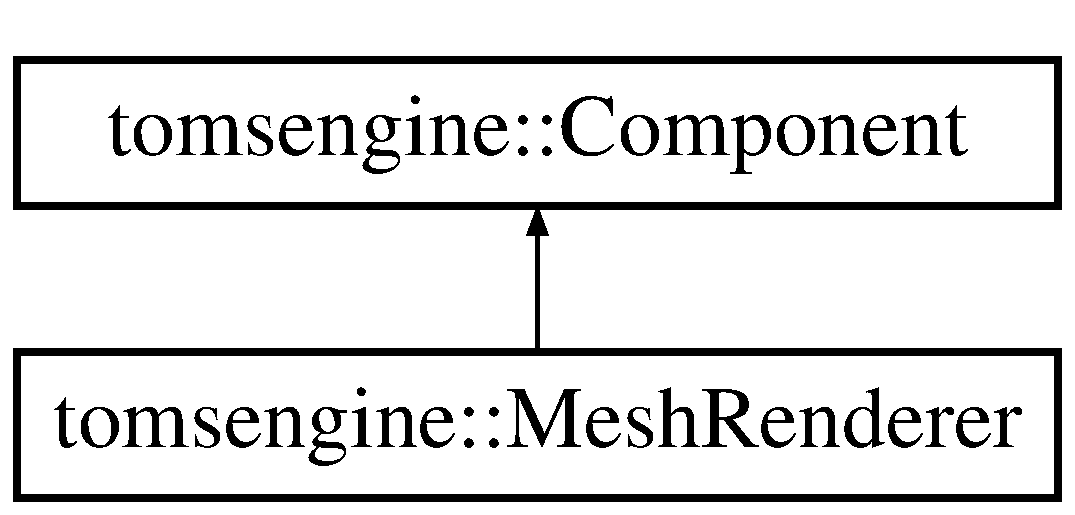
\includegraphics[height=2.000000cm]{classtomsengine_1_1_component}
\end{center}
\end{figure}
\subsection*{Public Member Functions}
\begin{DoxyCompactItemize}
\item 
virtual \mbox{\hyperlink{classtomsengine_1_1_component_a76e5a26860d666c9290057a140517f7e}{$\sim$\+Component}} ()
\item 
std\+::shared\+\_\+ptr$<$ \mbox{\hyperlink{classtomsengine_1_1_core}{Core}} $>$ \mbox{\hyperlink{classtomsengine_1_1_component_a377e917bf99c007b30ff12ceedd666ee}{get\+Core}} ()
\item 
std\+::shared\+\_\+ptr$<$ \mbox{\hyperlink{classtomsengine_1_1_entity}{Entity}} $>$ \mbox{\hyperlink{classtomsengine_1_1_component_a7091b67f11bc3b64db3d913e255a7840}{get\+Entity}} ()
\end{DoxyCompactItemize}
\subsection*{Friends}
\begin{DoxyCompactItemize}
\item 
class \mbox{\hyperlink{classtomsengine_1_1_component_a614439ccac0344926adc4c0165d64060}{Entity}}
\end{DoxyCompactItemize}


\subsection{Constructor \& Destructor Documentation}
\mbox{\Hypertarget{classtomsengine_1_1_component_a76e5a26860d666c9290057a140517f7e}\label{classtomsengine_1_1_component_a76e5a26860d666c9290057a140517f7e}} 
\index{tomsengine\+::\+Component@{tomsengine\+::\+Component}!````~Component@{$\sim$\+Component}}
\index{````~Component@{$\sim$\+Component}!tomsengine\+::\+Component@{tomsengine\+::\+Component}}
\subsubsection{\texorpdfstring{$\sim$\+Component()}{~Component()}}
{\footnotesize\ttfamily tomsengine\+::\+Component\+::$\sim$\+Component (\begin{DoxyParamCaption}{ }\end{DoxyParamCaption})\hspace{0.3cm}{\ttfamily [virtual]}}



\subsection{Member Function Documentation}
\mbox{\Hypertarget{classtomsengine_1_1_component_a377e917bf99c007b30ff12ceedd666ee}\label{classtomsengine_1_1_component_a377e917bf99c007b30ff12ceedd666ee}} 
\index{tomsengine\+::\+Component@{tomsengine\+::\+Component}!get\+Core@{get\+Core}}
\index{get\+Core@{get\+Core}!tomsengine\+::\+Component@{tomsengine\+::\+Component}}
\subsubsection{\texorpdfstring{get\+Core()}{getCore()}}
{\footnotesize\ttfamily std\+::shared\+\_\+ptr$<$ \mbox{\hyperlink{classtomsengine_1_1_core}{Core}} $>$ tomsengine\+::\+Component\+::get\+Core (\begin{DoxyParamCaption}{ }\end{DoxyParamCaption})}

\mbox{\Hypertarget{classtomsengine_1_1_component_a7091b67f11bc3b64db3d913e255a7840}\label{classtomsengine_1_1_component_a7091b67f11bc3b64db3d913e255a7840}} 
\index{tomsengine\+::\+Component@{tomsengine\+::\+Component}!get\+Entity@{get\+Entity}}
\index{get\+Entity@{get\+Entity}!tomsengine\+::\+Component@{tomsengine\+::\+Component}}
\subsubsection{\texorpdfstring{get\+Entity()}{getEntity()}}
{\footnotesize\ttfamily std\+::shared\+\_\+ptr$<$ \mbox{\hyperlink{classtomsengine_1_1_entity}{Entity}} $>$ tomsengine\+::\+Component\+::get\+Entity (\begin{DoxyParamCaption}{ }\end{DoxyParamCaption})}



\subsection{Friends And Related Function Documentation}
\mbox{\Hypertarget{classtomsengine_1_1_component_a614439ccac0344926adc4c0165d64060}\label{classtomsengine_1_1_component_a614439ccac0344926adc4c0165d64060}} 
\index{tomsengine\+::\+Component@{tomsengine\+::\+Component}!Entity@{Entity}}
\index{Entity@{Entity}!tomsengine\+::\+Component@{tomsengine\+::\+Component}}
\subsubsection{\texorpdfstring{Entity}{Entity}}
{\footnotesize\ttfamily friend class \mbox{\hyperlink{classtomsengine_1_1_entity}{Entity}}\hspace{0.3cm}{\ttfamily [friend]}}



The documentation for this class was generated from the following files\+:\begin{DoxyCompactItemize}
\item 
src/tomsengine/\mbox{\hyperlink{_component_8h}{Component.\+h}}\item 
src/tomsengine/\mbox{\hyperlink{_component_8cpp}{Component.\+cpp}}\end{DoxyCompactItemize}

\hypertarget{classtomsengine_1_1_core}{}\section{tomsengine\+:\+:Core Class Reference}
\label{classtomsengine_1_1_core}\index{tomsengine\+::\+Core@{tomsengine\+::\+Core}}


{\ttfamily \#include $<$Core.\+h$>$}

\subsection*{Public Member Functions}
\begin{DoxyCompactItemize}
\item 
\mbox{\hyperlink{classtomsengine_1_1_core_ad9b06b4a017762ce277c705d01922b5f}{Core}} ()
\item 
void \mbox{\hyperlink{classtomsengine_1_1_core_ad5e2c3d2900bef9155f9ee97eb9cdce4}{Start}} ()
\item 
void \mbox{\hyperlink{classtomsengine_1_1_core_a556fb0bd37ba3cef6a2b691f306538e6}{Stop}} ()
\item 
std\+::shared\+\_\+ptr$<$ \mbox{\hyperlink{classtomsengine_1_1_entity}{Entity}} $>$ \mbox{\hyperlink{classtomsengine_1_1_core_adefc590c422c9fa8559211fe8d0599de}{add\+Entity}} ()
\end{DoxyCompactItemize}


\subsection{Constructor \& Destructor Documentation}
\mbox{\Hypertarget{classtomsengine_1_1_core_ad9b06b4a017762ce277c705d01922b5f}\label{classtomsengine_1_1_core_ad9b06b4a017762ce277c705d01922b5f}} 
\index{tomsengine\+::\+Core@{tomsengine\+::\+Core}!Core@{Core}}
\index{Core@{Core}!tomsengine\+::\+Core@{tomsengine\+::\+Core}}
\subsubsection{\texorpdfstring{Core()}{Core()}}
{\footnotesize\ttfamily tomsengine\+::\+Core\+::\+Core (\begin{DoxyParamCaption}{ }\end{DoxyParamCaption})}



\subsection{Member Function Documentation}
\mbox{\Hypertarget{classtomsengine_1_1_core_adefc590c422c9fa8559211fe8d0599de}\label{classtomsengine_1_1_core_adefc590c422c9fa8559211fe8d0599de}} 
\index{tomsengine\+::\+Core@{tomsengine\+::\+Core}!add\+Entity@{add\+Entity}}
\index{add\+Entity@{add\+Entity}!tomsengine\+::\+Core@{tomsengine\+::\+Core}}
\subsubsection{\texorpdfstring{add\+Entity()}{addEntity()}}
{\footnotesize\ttfamily std\+::shared\+\_\+ptr$<$ \mbox{\hyperlink{classtomsengine_1_1_entity}{Entity}} $>$ tomsengine\+::\+Core\+::add\+Entity (\begin{DoxyParamCaption}{ }\end{DoxyParamCaption})}

\mbox{\Hypertarget{classtomsengine_1_1_core_ad5e2c3d2900bef9155f9ee97eb9cdce4}\label{classtomsengine_1_1_core_ad5e2c3d2900bef9155f9ee97eb9cdce4}} 
\index{tomsengine\+::\+Core@{tomsengine\+::\+Core}!Start@{Start}}
\index{Start@{Start}!tomsengine\+::\+Core@{tomsengine\+::\+Core}}
\subsubsection{\texorpdfstring{Start()}{Start()}}
{\footnotesize\ttfamily void tomsengine\+::\+Core\+::\+Start (\begin{DoxyParamCaption}{ }\end{DoxyParamCaption})}

\mbox{\Hypertarget{classtomsengine_1_1_core_a556fb0bd37ba3cef6a2b691f306538e6}\label{classtomsengine_1_1_core_a556fb0bd37ba3cef6a2b691f306538e6}} 
\index{tomsengine\+::\+Core@{tomsengine\+::\+Core}!Stop@{Stop}}
\index{Stop@{Stop}!tomsengine\+::\+Core@{tomsengine\+::\+Core}}
\subsubsection{\texorpdfstring{Stop()}{Stop()}}
{\footnotesize\ttfamily void tomsengine\+::\+Core\+::\+Stop (\begin{DoxyParamCaption}{ }\end{DoxyParamCaption})}



The documentation for this class was generated from the following files\+:\begin{DoxyCompactItemize}
\item 
src/tomsengine/\mbox{\hyperlink{_core_8h}{Core.\+h}}\item 
src/tomsengine/\mbox{\hyperlink{_core_8cpp}{Core.\+cpp}}\end{DoxyCompactItemize}

\hypertarget{classtomsengine_1_1_entity}{}\section{tomsengine\+:\+:Entity Class Reference}
\label{classtomsengine_1_1_entity}\index{tomsengine\+::\+Entity@{tomsengine\+::\+Entity}}


{\ttfamily \#include $<$Entity.\+h$>$}

\subsection*{Public Member Functions}
\begin{DoxyCompactItemize}
\item 
{\footnotesize template$<$typename T $>$ }\\std\+::shared\+\_\+ptr$<$ T $>$ \mbox{\hyperlink{classtomsengine_1_1_entity_ae21b5f4ee9d7b14e435c4e30158b31df}{get\+Component}} ()
\item 
{\footnotesize template$<$typename T $>$ }\\std\+::shared\+\_\+ptr$<$ T $>$ \mbox{\hyperlink{classtomsengine_1_1_entity_a1c7c295c7f130c529eaf606afa89500f}{add\+Component}} ()
\item 
{\footnotesize template$<$typename T , typename A $>$ }\\std\+::shared\+\_\+ptr$<$ T $>$ \mbox{\hyperlink{classtomsengine_1_1_entity_a6ac73653eb2a82ff00c799a3c2601cbd}{add\+Component}} (A a)
\item 
{\footnotesize template$<$typename T , typename A , typename B $>$ }\\std\+::shared\+\_\+ptr$<$ T $>$ \mbox{\hyperlink{classtomsengine_1_1_entity_a08a1874557bd871a4cd7484034b4196d}{add\+Component}} (A a, B b)
\item 
std\+::shared\+\_\+ptr$<$ \mbox{\hyperlink{classtomsengine_1_1_core}{Core}} $>$ \mbox{\hyperlink{classtomsengine_1_1_entity_a240e4cb523713f94bc26cfd965e9ddcf}{get\+Core}} ()
\end{DoxyCompactItemize}
\subsection*{Friends}
\begin{DoxyCompactItemize}
\item 
class \mbox{\hyperlink{classtomsengine_1_1_entity_a4107254ac74f90d4f91e810d755b98c2}{Core}}
\end{DoxyCompactItemize}


\subsection{Member Function Documentation}
\mbox{\Hypertarget{classtomsengine_1_1_entity_a1c7c295c7f130c529eaf606afa89500f}\label{classtomsengine_1_1_entity_a1c7c295c7f130c529eaf606afa89500f}} 
\index{tomsengine\+::\+Entity@{tomsengine\+::\+Entity}!add\+Component@{add\+Component}}
\index{add\+Component@{add\+Component}!tomsengine\+::\+Entity@{tomsengine\+::\+Entity}}
\subsubsection{\texorpdfstring{add\+Component()}{addComponent()}\hspace{0.1cm}{\footnotesize\ttfamily [1/3]}}
{\footnotesize\ttfamily template$<$typename T $>$ \\
std\+::shared\+\_\+ptr$<$T$>$ tomsengine\+::\+Entity\+::add\+Component (\begin{DoxyParamCaption}{ }\end{DoxyParamCaption})\hspace{0.3cm}{\ttfamily [inline]}}

\mbox{\Hypertarget{classtomsengine_1_1_entity_a6ac73653eb2a82ff00c799a3c2601cbd}\label{classtomsengine_1_1_entity_a6ac73653eb2a82ff00c799a3c2601cbd}} 
\index{tomsengine\+::\+Entity@{tomsengine\+::\+Entity}!add\+Component@{add\+Component}}
\index{add\+Component@{add\+Component}!tomsengine\+::\+Entity@{tomsengine\+::\+Entity}}
\subsubsection{\texorpdfstring{add\+Component()}{addComponent()}\hspace{0.1cm}{\footnotesize\ttfamily [2/3]}}
{\footnotesize\ttfamily template$<$typename T , typename A $>$ \\
std\+::shared\+\_\+ptr$<$T$>$ tomsengine\+::\+Entity\+::add\+Component (\begin{DoxyParamCaption}\item[{A}]{a }\end{DoxyParamCaption})\hspace{0.3cm}{\ttfamily [inline]}}

\mbox{\Hypertarget{classtomsengine_1_1_entity_a08a1874557bd871a4cd7484034b4196d}\label{classtomsengine_1_1_entity_a08a1874557bd871a4cd7484034b4196d}} 
\index{tomsengine\+::\+Entity@{tomsengine\+::\+Entity}!add\+Component@{add\+Component}}
\index{add\+Component@{add\+Component}!tomsengine\+::\+Entity@{tomsengine\+::\+Entity}}
\subsubsection{\texorpdfstring{add\+Component()}{addComponent()}\hspace{0.1cm}{\footnotesize\ttfamily [3/3]}}
{\footnotesize\ttfamily template$<$typename T , typename A , typename B $>$ \\
std\+::shared\+\_\+ptr$<$T$>$ tomsengine\+::\+Entity\+::add\+Component (\begin{DoxyParamCaption}\item[{A}]{a,  }\item[{B}]{b }\end{DoxyParamCaption})\hspace{0.3cm}{\ttfamily [inline]}}

\mbox{\Hypertarget{classtomsengine_1_1_entity_ae21b5f4ee9d7b14e435c4e30158b31df}\label{classtomsengine_1_1_entity_ae21b5f4ee9d7b14e435c4e30158b31df}} 
\index{tomsengine\+::\+Entity@{tomsengine\+::\+Entity}!get\+Component@{get\+Component}}
\index{get\+Component@{get\+Component}!tomsengine\+::\+Entity@{tomsengine\+::\+Entity}}
\subsubsection{\texorpdfstring{get\+Component()}{getComponent()}}
{\footnotesize\ttfamily template$<$typename T $>$ \\
std\+::shared\+\_\+ptr$<$T$>$ tomsengine\+::\+Entity\+::get\+Component (\begin{DoxyParamCaption}{ }\end{DoxyParamCaption})\hspace{0.3cm}{\ttfamily [inline]}}

\mbox{\Hypertarget{classtomsengine_1_1_entity_a240e4cb523713f94bc26cfd965e9ddcf}\label{classtomsengine_1_1_entity_a240e4cb523713f94bc26cfd965e9ddcf}} 
\index{tomsengine\+::\+Entity@{tomsengine\+::\+Entity}!get\+Core@{get\+Core}}
\index{get\+Core@{get\+Core}!tomsengine\+::\+Entity@{tomsengine\+::\+Entity}}
\subsubsection{\texorpdfstring{get\+Core()}{getCore()}}
{\footnotesize\ttfamily std\+::shared\+\_\+ptr$<$ \mbox{\hyperlink{classtomsengine_1_1_core}{Core}} $>$ tomsengine\+::\+Entity\+::get\+Core (\begin{DoxyParamCaption}{ }\end{DoxyParamCaption})}



\subsection{Friends And Related Function Documentation}
\mbox{\Hypertarget{classtomsengine_1_1_entity_a4107254ac74f90d4f91e810d755b98c2}\label{classtomsengine_1_1_entity_a4107254ac74f90d4f91e810d755b98c2}} 
\index{tomsengine\+::\+Entity@{tomsengine\+::\+Entity}!Core@{Core}}
\index{Core@{Core}!tomsengine\+::\+Entity@{tomsengine\+::\+Entity}}
\subsubsection{\texorpdfstring{Core}{Core}}
{\footnotesize\ttfamily friend class \mbox{\hyperlink{classtomsengine_1_1_core}{Core}}\hspace{0.3cm}{\ttfamily [friend]}}



The documentation for this class was generated from the following files\+:\begin{DoxyCompactItemize}
\item 
src/tomsengine/\mbox{\hyperlink{_entity_8h}{Entity.\+h}}\item 
src/tomsengine/\mbox{\hyperlink{_entity_8cpp}{Entity.\+cpp}}\end{DoxyCompactItemize}

\hypertarget{classtomsengine_1_1_mesh_renderer}{}\section{tomsengine\+:\+:Mesh\+Renderer Class Reference}
\label{classtomsengine_1_1_mesh_renderer}\index{tomsengine\+::\+Mesh\+Renderer@{tomsengine\+::\+Mesh\+Renderer}}


{\ttfamily \#include $<$Mesh\+Renderer.\+h$>$}

Inheritance diagram for tomsengine\+:\+:Mesh\+Renderer\+:\begin{figure}[H]
\begin{center}
\leavevmode
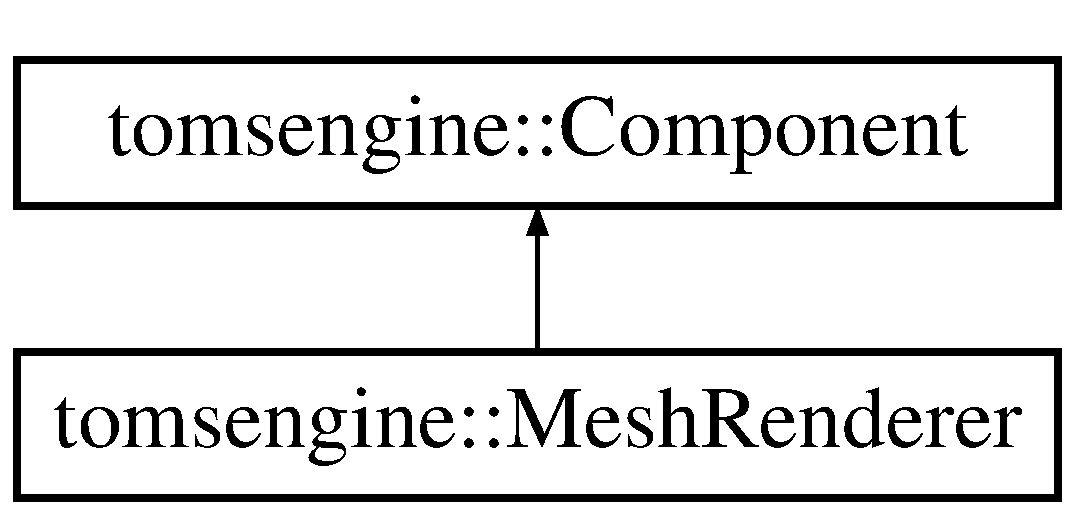
\includegraphics[height=2.000000cm]{classtomsengine_1_1_mesh_renderer}
\end{center}
\end{figure}
\subsection*{Public Member Functions}
\begin{DoxyCompactItemize}
\item 
void \mbox{\hyperlink{classtomsengine_1_1_mesh_renderer_a1811283a3daa29d1ee9f043fd99416a5}{on\+Init}} ()
\end{DoxyCompactItemize}


\subsection{Member Function Documentation}
\mbox{\Hypertarget{classtomsengine_1_1_mesh_renderer_a1811283a3daa29d1ee9f043fd99416a5}\label{classtomsengine_1_1_mesh_renderer_a1811283a3daa29d1ee9f043fd99416a5}} 
\index{tomsengine\+::\+Mesh\+Renderer@{tomsengine\+::\+Mesh\+Renderer}!on\+Init@{on\+Init}}
\index{on\+Init@{on\+Init}!tomsengine\+::\+Mesh\+Renderer@{tomsengine\+::\+Mesh\+Renderer}}
\subsubsection{\texorpdfstring{on\+Init()}{onInit()}}
{\footnotesize\ttfamily void tomsengine\+::\+Mesh\+Renderer\+::on\+Init (\begin{DoxyParamCaption}{ }\end{DoxyParamCaption})\hspace{0.3cm}{\ttfamily [virtual]}}



Reimplemented from \mbox{\hyperlink{classtomsengine_1_1_component}{tomsengine\+::\+Component}}.



The documentation for this class was generated from the following files\+:\begin{DoxyCompactItemize}
\item 
src/tomsengine/\mbox{\hyperlink{_mesh_renderer_8h}{Mesh\+Renderer.\+h}}\item 
src/tomsengine/\mbox{\hyperlink{_mesh_renderer_8cpp}{Mesh\+Renderer.\+cpp}}\end{DoxyCompactItemize}

\hypertarget{structtomsengine_1_1_sampler}{}\section{tomsengine\+:\+:Sampler Struct Reference}
\label{structtomsengine_1_1_sampler}\index{tomsengine\+::\+Sampler@{tomsengine\+::\+Sampler}}


{\ttfamily \#include $<$Shader.\+h$>$}

\subsection*{Public Attributes}
\begin{DoxyCompactItemize}
\item 
G\+Lint \mbox{\hyperlink{structtomsengine_1_1_sampler_a83b57ed27e47aa70ad7cf3f916e2dd49}{id}}
\item 
std\+::shared\+\_\+ptr$<$ \mbox{\hyperlink{classtomsengine_1_1_texture}{Texture}} $>$ \mbox{\hyperlink{structtomsengine_1_1_sampler_a30ac7eac57cbd1cbd791ca304fe3f9d5}{texture}}
\end{DoxyCompactItemize}


\subsection{Member Data Documentation}
\mbox{\Hypertarget{structtomsengine_1_1_sampler_a83b57ed27e47aa70ad7cf3f916e2dd49}\label{structtomsengine_1_1_sampler_a83b57ed27e47aa70ad7cf3f916e2dd49}} 
\index{tomsengine\+::\+Sampler@{tomsengine\+::\+Sampler}!id@{id}}
\index{id@{id}!tomsengine\+::\+Sampler@{tomsengine\+::\+Sampler}}
\subsubsection{\texorpdfstring{id}{id}}
{\footnotesize\ttfamily G\+Lint tomsengine\+::\+Sampler\+::id}

\mbox{\Hypertarget{structtomsengine_1_1_sampler_a30ac7eac57cbd1cbd791ca304fe3f9d5}\label{structtomsengine_1_1_sampler_a30ac7eac57cbd1cbd791ca304fe3f9d5}} 
\index{tomsengine\+::\+Sampler@{tomsengine\+::\+Sampler}!texture@{texture}}
\index{texture@{texture}!tomsengine\+::\+Sampler@{tomsengine\+::\+Sampler}}
\subsubsection{\texorpdfstring{texture}{texture}}
{\footnotesize\ttfamily std\+::shared\+\_\+ptr$<$\mbox{\hyperlink{classtomsengine_1_1_texture}{Texture}}$>$ tomsengine\+::\+Sampler\+::texture}



The documentation for this struct was generated from the following file\+:\begin{DoxyCompactItemize}
\item 
src/tomsengine/\mbox{\hyperlink{_shader_8h}{Shader.\+h}}\end{DoxyCompactItemize}

\hypertarget{classtomsengine_1_1_shader}{}\section{tomsengine\+:\+:Shader Class Reference}
\label{classtomsengine_1_1_shader}\index{tomsengine\+::\+Shader@{tomsengine\+::\+Shader}}


{\ttfamily \#include $<$Shader.\+h$>$}

\subsection*{Public Member Functions}
\begin{DoxyCompactItemize}
\item 
\mbox{\hyperlink{classtomsengine_1_1_shader_ac9d4712f35e8d3031973c49d8290b34d}{Shader}} (std\+::string vert, std\+::string frag)
\item 
void \mbox{\hyperlink{classtomsengine_1_1_shader_af63fb3f1221631fd17ee7e814eec579c}{draw}} (std\+::shared\+\_\+ptr$<$ \mbox{\hyperlink{classtomsengine_1_1_vertex_array}{Vertex\+Array}} $>$ vertex\+Array)
\item 
void \mbox{\hyperlink{classtomsengine_1_1_shader_a2bcc5799fdbed02cf8fc57a2db0bf1f2}{set\+Uniform}} (std\+::string uniform, glm\+::vec4 value)
\item 
void \mbox{\hyperlink{classtomsengine_1_1_shader_ac2273cc9e24be079c10bf957236044be}{set\+Uniform}} (std\+::string uniform, float value)
\item 
void \mbox{\hyperlink{classtomsengine_1_1_shader_ae17443671c6e427199bc3da08b790438}{set\+Uniform}} (std\+::string uniform, glm\+::mat4 value)
\item 
void \mbox{\hyperlink{classtomsengine_1_1_shader_a604bd6c3971d78104253a6ee04421cbd}{set\+Uniform}} (std\+::string uniform, std\+::shared\+\_\+ptr$<$ \mbox{\hyperlink{classtomsengine_1_1_texture}{Texture}} $>$ texture)
\item 
G\+Luint \mbox{\hyperlink{classtomsengine_1_1_shader_aa7f2be24efa50e52bb3dfe03551e3792}{get\+Id}} ()
\end{DoxyCompactItemize}


\subsection{Constructor \& Destructor Documentation}
\mbox{\Hypertarget{classtomsengine_1_1_shader_ac9d4712f35e8d3031973c49d8290b34d}\label{classtomsengine_1_1_shader_ac9d4712f35e8d3031973c49d8290b34d}} 
\index{tomsengine\+::\+Shader@{tomsengine\+::\+Shader}!Shader@{Shader}}
\index{Shader@{Shader}!tomsengine\+::\+Shader@{tomsengine\+::\+Shader}}
\subsubsection{\texorpdfstring{Shader()}{Shader()}}
{\footnotesize\ttfamily tomsengine\+::\+Shader\+::\+Shader (\begin{DoxyParamCaption}\item[{std\+::string}]{vert,  }\item[{std\+::string}]{frag }\end{DoxyParamCaption})}



\subsection{Member Function Documentation}
\mbox{\Hypertarget{classtomsengine_1_1_shader_af63fb3f1221631fd17ee7e814eec579c}\label{classtomsengine_1_1_shader_af63fb3f1221631fd17ee7e814eec579c}} 
\index{tomsengine\+::\+Shader@{tomsengine\+::\+Shader}!draw@{draw}}
\index{draw@{draw}!tomsengine\+::\+Shader@{tomsengine\+::\+Shader}}
\subsubsection{\texorpdfstring{draw()}{draw()}}
{\footnotesize\ttfamily void tomsengine\+::\+Shader\+::draw (\begin{DoxyParamCaption}\item[{std\+::shared\+\_\+ptr$<$ \mbox{\hyperlink{classtomsengine_1_1_vertex_array}{Vertex\+Array}} $>$}]{vertex\+Array }\end{DoxyParamCaption})}

\mbox{\Hypertarget{classtomsengine_1_1_shader_aa7f2be24efa50e52bb3dfe03551e3792}\label{classtomsengine_1_1_shader_aa7f2be24efa50e52bb3dfe03551e3792}} 
\index{tomsengine\+::\+Shader@{tomsengine\+::\+Shader}!get\+Id@{get\+Id}}
\index{get\+Id@{get\+Id}!tomsengine\+::\+Shader@{tomsengine\+::\+Shader}}
\subsubsection{\texorpdfstring{get\+Id()}{getId()}}
{\footnotesize\ttfamily G\+Luint tomsengine\+::\+Shader\+::get\+Id (\begin{DoxyParamCaption}{ }\end{DoxyParamCaption})}

\mbox{\Hypertarget{classtomsengine_1_1_shader_a2bcc5799fdbed02cf8fc57a2db0bf1f2}\label{classtomsengine_1_1_shader_a2bcc5799fdbed02cf8fc57a2db0bf1f2}} 
\index{tomsengine\+::\+Shader@{tomsengine\+::\+Shader}!set\+Uniform@{set\+Uniform}}
\index{set\+Uniform@{set\+Uniform}!tomsengine\+::\+Shader@{tomsengine\+::\+Shader}}
\subsubsection{\texorpdfstring{set\+Uniform()}{setUniform()}\hspace{0.1cm}{\footnotesize\ttfamily [1/4]}}
{\footnotesize\ttfamily void tomsengine\+::\+Shader\+::set\+Uniform (\begin{DoxyParamCaption}\item[{std\+::string}]{uniform,  }\item[{glm\+::vec4}]{value }\end{DoxyParamCaption})}

\mbox{\Hypertarget{classtomsengine_1_1_shader_ac2273cc9e24be079c10bf957236044be}\label{classtomsengine_1_1_shader_ac2273cc9e24be079c10bf957236044be}} 
\index{tomsengine\+::\+Shader@{tomsengine\+::\+Shader}!set\+Uniform@{set\+Uniform}}
\index{set\+Uniform@{set\+Uniform}!tomsengine\+::\+Shader@{tomsengine\+::\+Shader}}
\subsubsection{\texorpdfstring{set\+Uniform()}{setUniform()}\hspace{0.1cm}{\footnotesize\ttfamily [2/4]}}
{\footnotesize\ttfamily void tomsengine\+::\+Shader\+::set\+Uniform (\begin{DoxyParamCaption}\item[{std\+::string}]{uniform,  }\item[{float}]{value }\end{DoxyParamCaption})}

\mbox{\Hypertarget{classtomsengine_1_1_shader_ae17443671c6e427199bc3da08b790438}\label{classtomsengine_1_1_shader_ae17443671c6e427199bc3da08b790438}} 
\index{tomsengine\+::\+Shader@{tomsengine\+::\+Shader}!set\+Uniform@{set\+Uniform}}
\index{set\+Uniform@{set\+Uniform}!tomsengine\+::\+Shader@{tomsengine\+::\+Shader}}
\subsubsection{\texorpdfstring{set\+Uniform()}{setUniform()}\hspace{0.1cm}{\footnotesize\ttfamily [3/4]}}
{\footnotesize\ttfamily void tomsengine\+::\+Shader\+::set\+Uniform (\begin{DoxyParamCaption}\item[{std\+::string}]{uniform,  }\item[{glm\+::mat4}]{value }\end{DoxyParamCaption})}

\mbox{\Hypertarget{classtomsengine_1_1_shader_a604bd6c3971d78104253a6ee04421cbd}\label{classtomsengine_1_1_shader_a604bd6c3971d78104253a6ee04421cbd}} 
\index{tomsengine\+::\+Shader@{tomsengine\+::\+Shader}!set\+Uniform@{set\+Uniform}}
\index{set\+Uniform@{set\+Uniform}!tomsengine\+::\+Shader@{tomsengine\+::\+Shader}}
\subsubsection{\texorpdfstring{set\+Uniform()}{setUniform()}\hspace{0.1cm}{\footnotesize\ttfamily [4/4]}}
{\footnotesize\ttfamily void tomsengine\+::\+Shader\+::set\+Uniform (\begin{DoxyParamCaption}\item[{std\+::string}]{uniform,  }\item[{std\+::shared\+\_\+ptr$<$ \mbox{\hyperlink{classtomsengine_1_1_texture}{Texture}} $>$}]{texture }\end{DoxyParamCaption})}



The documentation for this class was generated from the following files\+:\begin{DoxyCompactItemize}
\item 
src/tomsengine/\mbox{\hyperlink{_shader_8h}{Shader.\+h}}\item 
src/tomsengine/\mbox{\hyperlink{_shader_8cpp}{Shader.\+cpp}}\end{DoxyCompactItemize}

\hypertarget{classtomsengine_1_1_texture}{}\section{tomsengine\+:\+:Texture Class Reference}
\label{classtomsengine_1_1_texture}\index{tomsengine\+::\+Texture@{tomsengine\+::\+Texture}}


{\ttfamily \#include $<$Texture.\+h$>$}

\subsection*{Public Member Functions}
\begin{DoxyCompactItemize}
\item 
\mbox{\hyperlink{classtomsengine_1_1_texture_a0afe8db9c4f2d4ffc55430f1ed92e053}{Texture}} (std\+::string path)
\item 
glm\+::vec2 \mbox{\hyperlink{classtomsengine_1_1_texture_a270a5d664501ca0e7843a737508dbba5}{get\+Size}} ()
\item 
G\+Luint \mbox{\hyperlink{classtomsengine_1_1_texture_a9224651f86e573dd31436d919258dc03}{get\+Id}} ()
\end{DoxyCompactItemize}


\subsection{Constructor \& Destructor Documentation}
\mbox{\Hypertarget{classtomsengine_1_1_texture_a0afe8db9c4f2d4ffc55430f1ed92e053}\label{classtomsengine_1_1_texture_a0afe8db9c4f2d4ffc55430f1ed92e053}} 
\index{tomsengine\+::\+Texture@{tomsengine\+::\+Texture}!Texture@{Texture}}
\index{Texture@{Texture}!tomsengine\+::\+Texture@{tomsengine\+::\+Texture}}
\subsubsection{\texorpdfstring{Texture()}{Texture()}}
{\footnotesize\ttfamily tomsengine\+::\+Texture\+::\+Texture (\begin{DoxyParamCaption}\item[{std\+::string}]{path }\end{DoxyParamCaption})}



\subsection{Member Function Documentation}
\mbox{\Hypertarget{classtomsengine_1_1_texture_a9224651f86e573dd31436d919258dc03}\label{classtomsengine_1_1_texture_a9224651f86e573dd31436d919258dc03}} 
\index{tomsengine\+::\+Texture@{tomsengine\+::\+Texture}!get\+Id@{get\+Id}}
\index{get\+Id@{get\+Id}!tomsengine\+::\+Texture@{tomsengine\+::\+Texture}}
\subsubsection{\texorpdfstring{get\+Id()}{getId()}}
{\footnotesize\ttfamily G\+Luint tomsengine\+::\+Texture\+::get\+Id (\begin{DoxyParamCaption}{ }\end{DoxyParamCaption})}

\mbox{\Hypertarget{classtomsengine_1_1_texture_a270a5d664501ca0e7843a737508dbba5}\label{classtomsengine_1_1_texture_a270a5d664501ca0e7843a737508dbba5}} 
\index{tomsengine\+::\+Texture@{tomsengine\+::\+Texture}!get\+Size@{get\+Size}}
\index{get\+Size@{get\+Size}!tomsengine\+::\+Texture@{tomsengine\+::\+Texture}}
\subsubsection{\texorpdfstring{get\+Size()}{getSize()}}
{\footnotesize\ttfamily glm\+::vec2 tomsengine\+::\+Texture\+::get\+Size (\begin{DoxyParamCaption}{ }\end{DoxyParamCaption})}



The documentation for this class was generated from the following files\+:\begin{DoxyCompactItemize}
\item 
src/tomsengine/\mbox{\hyperlink{_texture_8h}{Texture.\+h}}\item 
src/tomsengine/\mbox{\hyperlink{_texture_8cpp}{Texture.\+cpp}}\end{DoxyCompactItemize}

\hypertarget{classtomsengine_1_1_vertex_array}{}\section{tomsengine\+:\+:Vertex\+Array Class Reference}
\label{classtomsengine_1_1_vertex_array}\index{tomsengine\+::\+Vertex\+Array@{tomsengine\+::\+Vertex\+Array}}


{\ttfamily \#include $<$Vertex\+Array.\+h$>$}

\subsection*{Public Member Functions}
\begin{DoxyCompactItemize}
\item 
\mbox{\hyperlink{classtomsengine_1_1_vertex_array_a3303a68dab144005078e112096690361}{Vertex\+Array}} ()
\item 
\mbox{\hyperlink{classtomsengine_1_1_vertex_array_ab8e0cf34f040957b0293594218c15fea}{Vertex\+Array}} (std\+::string path)
\item 
void \mbox{\hyperlink{classtomsengine_1_1_vertex_array_a874821cb99cd06bd58eb9a3e552c54aa}{set\+Buffer}} (std\+::string attribute, \mbox{\hyperlink{classtomsengine_1_1_vertex_buffer}{Vertex\+Buffer}} $\ast$buffer)
\item 
int \mbox{\hyperlink{classtomsengine_1_1_vertex_array_a9084bfe0cfa2dc86a2322079b5ed13d4}{get\+Vertex\+Count}} ()
\item 
G\+Luint \mbox{\hyperlink{classtomsengine_1_1_vertex_array_a6b5d7767d60c35451a34237cf36f0166}{get\+Id}} ()
\end{DoxyCompactItemize}


\subsection{Constructor \& Destructor Documentation}
\mbox{\Hypertarget{classtomsengine_1_1_vertex_array_a3303a68dab144005078e112096690361}\label{classtomsengine_1_1_vertex_array_a3303a68dab144005078e112096690361}} 
\index{tomsengine\+::\+Vertex\+Array@{tomsengine\+::\+Vertex\+Array}!Vertex\+Array@{Vertex\+Array}}
\index{Vertex\+Array@{Vertex\+Array}!tomsengine\+::\+Vertex\+Array@{tomsengine\+::\+Vertex\+Array}}
\subsubsection{\texorpdfstring{Vertex\+Array()}{VertexArray()}\hspace{0.1cm}{\footnotesize\ttfamily [1/2]}}
{\footnotesize\ttfamily tomsengine\+::\+Vertex\+Array\+::\+Vertex\+Array (\begin{DoxyParamCaption}{ }\end{DoxyParamCaption})}

\mbox{\Hypertarget{classtomsengine_1_1_vertex_array_ab8e0cf34f040957b0293594218c15fea}\label{classtomsengine_1_1_vertex_array_ab8e0cf34f040957b0293594218c15fea}} 
\index{tomsengine\+::\+Vertex\+Array@{tomsengine\+::\+Vertex\+Array}!Vertex\+Array@{Vertex\+Array}}
\index{Vertex\+Array@{Vertex\+Array}!tomsengine\+::\+Vertex\+Array@{tomsengine\+::\+Vertex\+Array}}
\subsubsection{\texorpdfstring{Vertex\+Array()}{VertexArray()}\hspace{0.1cm}{\footnotesize\ttfamily [2/2]}}
{\footnotesize\ttfamily tomsengine\+::\+Vertex\+Array\+::\+Vertex\+Array (\begin{DoxyParamCaption}\item[{std\+::string}]{path }\end{DoxyParamCaption})}



\subsection{Member Function Documentation}
\mbox{\Hypertarget{classtomsengine_1_1_vertex_array_a6b5d7767d60c35451a34237cf36f0166}\label{classtomsengine_1_1_vertex_array_a6b5d7767d60c35451a34237cf36f0166}} 
\index{tomsengine\+::\+Vertex\+Array@{tomsengine\+::\+Vertex\+Array}!get\+Id@{get\+Id}}
\index{get\+Id@{get\+Id}!tomsengine\+::\+Vertex\+Array@{tomsengine\+::\+Vertex\+Array}}
\subsubsection{\texorpdfstring{get\+Id()}{getId()}}
{\footnotesize\ttfamily G\+Luint tomsengine\+::\+Vertex\+Array\+::get\+Id (\begin{DoxyParamCaption}{ }\end{DoxyParamCaption})}

\mbox{\Hypertarget{classtomsengine_1_1_vertex_array_a9084bfe0cfa2dc86a2322079b5ed13d4}\label{classtomsengine_1_1_vertex_array_a9084bfe0cfa2dc86a2322079b5ed13d4}} 
\index{tomsengine\+::\+Vertex\+Array@{tomsengine\+::\+Vertex\+Array}!get\+Vertex\+Count@{get\+Vertex\+Count}}
\index{get\+Vertex\+Count@{get\+Vertex\+Count}!tomsengine\+::\+Vertex\+Array@{tomsengine\+::\+Vertex\+Array}}
\subsubsection{\texorpdfstring{get\+Vertex\+Count()}{getVertexCount()}}
{\footnotesize\ttfamily int tomsengine\+::\+Vertex\+Array\+::get\+Vertex\+Count (\begin{DoxyParamCaption}{ }\end{DoxyParamCaption})}

\mbox{\Hypertarget{classtomsengine_1_1_vertex_array_a874821cb99cd06bd58eb9a3e552c54aa}\label{classtomsengine_1_1_vertex_array_a874821cb99cd06bd58eb9a3e552c54aa}} 
\index{tomsengine\+::\+Vertex\+Array@{tomsengine\+::\+Vertex\+Array}!set\+Buffer@{set\+Buffer}}
\index{set\+Buffer@{set\+Buffer}!tomsengine\+::\+Vertex\+Array@{tomsengine\+::\+Vertex\+Array}}
\subsubsection{\texorpdfstring{set\+Buffer()}{setBuffer()}}
{\footnotesize\ttfamily void tomsengine\+::\+Vertex\+Array\+::set\+Buffer (\begin{DoxyParamCaption}\item[{std\+::string}]{attribute,  }\item[{\mbox{\hyperlink{classtomsengine_1_1_vertex_buffer}{Vertex\+Buffer}} $\ast$}]{buffer }\end{DoxyParamCaption})}



The documentation for this class was generated from the following files\+:\begin{DoxyCompactItemize}
\item 
src/tomsengine/\mbox{\hyperlink{_vertex_array_8h}{Vertex\+Array.\+h}}\item 
src/tomsengine/\mbox{\hyperlink{_vertex_array_8cpp}{Vertex\+Array.\+cpp}}\end{DoxyCompactItemize}

\hypertarget{classtomsengine_1_1_vertex_buffer}{}\section{tomsengine\+:\+:Vertex\+Buffer Class Reference}
\label{classtomsengine_1_1_vertex_buffer}\index{tomsengine\+::\+Vertex\+Buffer@{tomsengine\+::\+Vertex\+Buffer}}


{\ttfamily \#include $<$Vertex\+Buffer.\+h$>$}

\subsection*{Public Member Functions}
\begin{DoxyCompactItemize}
\item 
\mbox{\hyperlink{classtomsengine_1_1_vertex_buffer_abca71af12ff47c217e20339b7e01de55}{Vertex\+Buffer}} ()
\item 
void \mbox{\hyperlink{classtomsengine_1_1_vertex_buffer_abae8451195dd422b63984bbdc6be0057}{add}} (glm\+::vec2 value)
\item 
void \mbox{\hyperlink{classtomsengine_1_1_vertex_buffer_ab2625dd07630e3c688b2eb0850f8e056}{add}} (glm\+::vec3 value)
\item 
void \mbox{\hyperlink{classtomsengine_1_1_vertex_buffer_ae82b34dbc0446ba909d8f77623151c77}{add}} (glm\+::vec4 value)
\item 
int \mbox{\hyperlink{classtomsengine_1_1_vertex_buffer_a8c14b28f3a7e8be817fe96fee3eff267}{get\+Components}} ()
\item 
int \mbox{\hyperlink{classtomsengine_1_1_vertex_buffer_ae8896eeaab9d4602d4d4f7db3d583d87}{get\+Data\+Size}} ()
\item 
G\+Luint \mbox{\hyperlink{classtomsengine_1_1_vertex_buffer_a2a50925ab34c9084ccb164188fcf35b2}{get\+Id}} ()
\end{DoxyCompactItemize}


\subsection{Constructor \& Destructor Documentation}
\mbox{\Hypertarget{classtomsengine_1_1_vertex_buffer_abca71af12ff47c217e20339b7e01de55}\label{classtomsengine_1_1_vertex_buffer_abca71af12ff47c217e20339b7e01de55}} 
\index{tomsengine\+::\+Vertex\+Buffer@{tomsengine\+::\+Vertex\+Buffer}!Vertex\+Buffer@{Vertex\+Buffer}}
\index{Vertex\+Buffer@{Vertex\+Buffer}!tomsengine\+::\+Vertex\+Buffer@{tomsengine\+::\+Vertex\+Buffer}}
\subsubsection{\texorpdfstring{Vertex\+Buffer()}{VertexBuffer()}}
{\footnotesize\ttfamily tomsengine\+::\+Vertex\+Buffer\+::\+Vertex\+Buffer (\begin{DoxyParamCaption}{ }\end{DoxyParamCaption})}



\subsection{Member Function Documentation}
\mbox{\Hypertarget{classtomsengine_1_1_vertex_buffer_abae8451195dd422b63984bbdc6be0057}\label{classtomsengine_1_1_vertex_buffer_abae8451195dd422b63984bbdc6be0057}} 
\index{tomsengine\+::\+Vertex\+Buffer@{tomsengine\+::\+Vertex\+Buffer}!add@{add}}
\index{add@{add}!tomsengine\+::\+Vertex\+Buffer@{tomsengine\+::\+Vertex\+Buffer}}
\subsubsection{\texorpdfstring{add()}{add()}\hspace{0.1cm}{\footnotesize\ttfamily [1/3]}}
{\footnotesize\ttfamily void tomsengine\+::\+Vertex\+Buffer\+::add (\begin{DoxyParamCaption}\item[{glm\+::vec2}]{value }\end{DoxyParamCaption})}

\mbox{\Hypertarget{classtomsengine_1_1_vertex_buffer_ab2625dd07630e3c688b2eb0850f8e056}\label{classtomsengine_1_1_vertex_buffer_ab2625dd07630e3c688b2eb0850f8e056}} 
\index{tomsengine\+::\+Vertex\+Buffer@{tomsengine\+::\+Vertex\+Buffer}!add@{add}}
\index{add@{add}!tomsengine\+::\+Vertex\+Buffer@{tomsengine\+::\+Vertex\+Buffer}}
\subsubsection{\texorpdfstring{add()}{add()}\hspace{0.1cm}{\footnotesize\ttfamily [2/3]}}
{\footnotesize\ttfamily void tomsengine\+::\+Vertex\+Buffer\+::add (\begin{DoxyParamCaption}\item[{glm\+::vec3}]{value }\end{DoxyParamCaption})}

\mbox{\Hypertarget{classtomsengine_1_1_vertex_buffer_ae82b34dbc0446ba909d8f77623151c77}\label{classtomsengine_1_1_vertex_buffer_ae82b34dbc0446ba909d8f77623151c77}} 
\index{tomsengine\+::\+Vertex\+Buffer@{tomsengine\+::\+Vertex\+Buffer}!add@{add}}
\index{add@{add}!tomsengine\+::\+Vertex\+Buffer@{tomsengine\+::\+Vertex\+Buffer}}
\subsubsection{\texorpdfstring{add()}{add()}\hspace{0.1cm}{\footnotesize\ttfamily [3/3]}}
{\footnotesize\ttfamily void tomsengine\+::\+Vertex\+Buffer\+::add (\begin{DoxyParamCaption}\item[{glm\+::vec4}]{value }\end{DoxyParamCaption})}

\mbox{\Hypertarget{classtomsengine_1_1_vertex_buffer_a8c14b28f3a7e8be817fe96fee3eff267}\label{classtomsengine_1_1_vertex_buffer_a8c14b28f3a7e8be817fe96fee3eff267}} 
\index{tomsengine\+::\+Vertex\+Buffer@{tomsengine\+::\+Vertex\+Buffer}!get\+Components@{get\+Components}}
\index{get\+Components@{get\+Components}!tomsengine\+::\+Vertex\+Buffer@{tomsengine\+::\+Vertex\+Buffer}}
\subsubsection{\texorpdfstring{get\+Components()}{getComponents()}}
{\footnotesize\ttfamily int tomsengine\+::\+Vertex\+Buffer\+::get\+Components (\begin{DoxyParamCaption}{ }\end{DoxyParamCaption})}

\mbox{\Hypertarget{classtomsengine_1_1_vertex_buffer_ae8896eeaab9d4602d4d4f7db3d583d87}\label{classtomsengine_1_1_vertex_buffer_ae8896eeaab9d4602d4d4f7db3d583d87}} 
\index{tomsengine\+::\+Vertex\+Buffer@{tomsengine\+::\+Vertex\+Buffer}!get\+Data\+Size@{get\+Data\+Size}}
\index{get\+Data\+Size@{get\+Data\+Size}!tomsengine\+::\+Vertex\+Buffer@{tomsengine\+::\+Vertex\+Buffer}}
\subsubsection{\texorpdfstring{get\+Data\+Size()}{getDataSize()}}
{\footnotesize\ttfamily int tomsengine\+::\+Vertex\+Buffer\+::get\+Data\+Size (\begin{DoxyParamCaption}{ }\end{DoxyParamCaption})}

\mbox{\Hypertarget{classtomsengine_1_1_vertex_buffer_a2a50925ab34c9084ccb164188fcf35b2}\label{classtomsengine_1_1_vertex_buffer_a2a50925ab34c9084ccb164188fcf35b2}} 
\index{tomsengine\+::\+Vertex\+Buffer@{tomsengine\+::\+Vertex\+Buffer}!get\+Id@{get\+Id}}
\index{get\+Id@{get\+Id}!tomsengine\+::\+Vertex\+Buffer@{tomsengine\+::\+Vertex\+Buffer}}
\subsubsection{\texorpdfstring{get\+Id()}{getId()}}
{\footnotesize\ttfamily G\+Luint tomsengine\+::\+Vertex\+Buffer\+::get\+Id (\begin{DoxyParamCaption}{ }\end{DoxyParamCaption})}



The documentation for this class was generated from the following files\+:\begin{DoxyCompactItemize}
\item 
src/tomsengine/\mbox{\hyperlink{_vertex_buffer_8h}{Vertex\+Buffer.\+h}}\item 
src/tomsengine/\mbox{\hyperlink{_vertex_buffer_8cpp}{Vertex\+Buffer.\+cpp}}\end{DoxyCompactItemize}

\chapter{File Documentation}
\hypertarget{_audio_8cpp}{}\section{src/tomsengine/\+Audio.cpp File Reference}
\label{_audio_8cpp}\index{src/tomsengine/\+Audio.\+cpp@{src/tomsengine/\+Audio.\+cpp}}
{\ttfamily \#include \char`\"{}Audio.\+h\char`\"{}}\newline
{\ttfamily \#include $<$A\+L/al.\+h$>$}\newline
{\ttfamily \#include $<$vorbis/vorbisfile.\+h$>$}\newline
{\ttfamily \#include $<$iostream$>$}\newline
{\ttfamily \#include $<$vector$>$}\newline
\subsection*{Classes}
\begin{DoxyCompactItemize}
\item 
struct \mbox{\hyperlink{structtomsengine_1_1_audio_impl}{tomsengine\+::\+Audio\+Impl}}
\end{DoxyCompactItemize}
\subsection*{Namespaces}
\begin{DoxyCompactItemize}
\item 
 \mbox{\hyperlink{namespacetomsengine}{tomsengine}}
\end{DoxyCompactItemize}

\hypertarget{_audio_8h}{}\section{src/tomsengine/\+Audio.h File Reference}
\label{_audio_8h}\index{src/tomsengine/\+Audio.\+h@{src/tomsengine/\+Audio.\+h}}
{\ttfamily \#include $<$memory$>$}\newline
{\ttfamily \#include $<$string$>$}\newline
\subsection*{Classes}
\begin{DoxyCompactItemize}
\item 
class \mbox{\hyperlink{classtomsengine_1_1_audio}{tomsengine\+::\+Audio}}
\end{DoxyCompactItemize}
\subsection*{Namespaces}
\begin{DoxyCompactItemize}
\item 
 \mbox{\hyperlink{namespacetomsengine}{tomsengine}}
\end{DoxyCompactItemize}

\hypertarget{_component_8cpp}{}\section{src/tomsengine/\+Component.cpp File Reference}
\label{_component_8cpp}\index{src/tomsengine/\+Component.\+cpp@{src/tomsengine/\+Component.\+cpp}}
{\ttfamily \#include \char`\"{}Component.\+h\char`\"{}}\newline
{\ttfamily \#include \char`\"{}Entity.\+h\char`\"{}}\newline
\subsection*{Namespaces}
\begin{DoxyCompactItemize}
\item 
 \mbox{\hyperlink{namespacetomsengine}{tomsengine}}
\end{DoxyCompactItemize}

\hypertarget{_component_8h}{}\section{src/tomsengine/\+Component.h File Reference}
\label{_component_8h}\index{src/tomsengine/\+Component.\+h@{src/tomsengine/\+Component.\+h}}
{\ttfamily \#include $<$memory$>$}\newline
\subsection*{Classes}
\begin{DoxyCompactItemize}
\item 
class \mbox{\hyperlink{classtomsengine_1_1_component}{tomsengine\+::\+Component}}
\end{DoxyCompactItemize}
\subsection*{Namespaces}
\begin{DoxyCompactItemize}
\item 
 \mbox{\hyperlink{namespacetomsengine}{tomsengine}}
\end{DoxyCompactItemize}

\hypertarget{_core_8cpp}{}\section{src/tomsengine/\+Core.cpp File Reference}
\label{_core_8cpp}\index{src/tomsengine/\+Core.\+cpp@{src/tomsengine/\+Core.\+cpp}}
{\ttfamily \#include \char`\"{}Core.\+h\char`\"{}}\newline
{\ttfamily \#include \char`\"{}Entity.\+h\char`\"{}}\newline
{\ttfamily \#include $<$G\+L/glew.\+h$>$}\newline
\subsection*{Namespaces}
\begin{DoxyCompactItemize}
\item 
 \mbox{\hyperlink{namespacetomsengine}{tomsengine}}
\end{DoxyCompactItemize}
\subsection*{Macros}
\begin{DoxyCompactItemize}
\item 
\#define \mbox{\hyperlink{_core_8cpp_a498d9f026138406895e9a34b504ac6a6}{W\+I\+N\+D\+O\+W\+\_\+\+W\+I\+D\+TH}}~1200
\item 
\#define \mbox{\hyperlink{_core_8cpp_a5473cf64fa979b48335079c99532e243}{W\+I\+N\+D\+O\+W\+\_\+\+H\+E\+I\+G\+HT}}~800
\end{DoxyCompactItemize}


\subsection{Macro Definition Documentation}
\mbox{\Hypertarget{_core_8cpp_a5473cf64fa979b48335079c99532e243}\label{_core_8cpp_a5473cf64fa979b48335079c99532e243}} 
\index{Core.\+cpp@{Core.\+cpp}!W\+I\+N\+D\+O\+W\+\_\+\+H\+E\+I\+G\+HT@{W\+I\+N\+D\+O\+W\+\_\+\+H\+E\+I\+G\+HT}}
\index{W\+I\+N\+D\+O\+W\+\_\+\+H\+E\+I\+G\+HT@{W\+I\+N\+D\+O\+W\+\_\+\+H\+E\+I\+G\+HT}!Core.\+cpp@{Core.\+cpp}}
\subsubsection{\texorpdfstring{W\+I\+N\+D\+O\+W\+\_\+\+H\+E\+I\+G\+HT}{WINDOW\_HEIGHT}}
{\footnotesize\ttfamily \#define W\+I\+N\+D\+O\+W\+\_\+\+H\+E\+I\+G\+HT~800}

\mbox{\Hypertarget{_core_8cpp_a498d9f026138406895e9a34b504ac6a6}\label{_core_8cpp_a498d9f026138406895e9a34b504ac6a6}} 
\index{Core.\+cpp@{Core.\+cpp}!W\+I\+N\+D\+O\+W\+\_\+\+W\+I\+D\+TH@{W\+I\+N\+D\+O\+W\+\_\+\+W\+I\+D\+TH}}
\index{W\+I\+N\+D\+O\+W\+\_\+\+W\+I\+D\+TH@{W\+I\+N\+D\+O\+W\+\_\+\+W\+I\+D\+TH}!Core.\+cpp@{Core.\+cpp}}
\subsubsection{\texorpdfstring{W\+I\+N\+D\+O\+W\+\_\+\+W\+I\+D\+TH}{WINDOW\_WIDTH}}
{\footnotesize\ttfamily \#define W\+I\+N\+D\+O\+W\+\_\+\+W\+I\+D\+TH~1200}


\hypertarget{_core_8h}{}\section{src/tomsengine/\+Core.h File Reference}
\label{_core_8h}\index{src/tomsengine/\+Core.\+h@{src/tomsengine/\+Core.\+h}}
{\ttfamily \#include $<$G\+L/glew.\+h$>$}\newline
{\ttfamily \#include $<$S\+D\+L2/\+S\+D\+L.\+h$>$}\newline
{\ttfamily \#include $<$A\+L/al.\+h$>$}\newline
{\ttfamily \#include $<$A\+L/alc.\+h$>$}\newline
{\ttfamily \#include $<$memory$>$}\newline
{\ttfamily \#include $<$vector$>$}\newline
\subsection*{Classes}
\begin{DoxyCompactItemize}
\item 
class \mbox{\hyperlink{classtomsengine_1_1_core}{tomsengine\+::\+Core}}
\end{DoxyCompactItemize}
\subsection*{Namespaces}
\begin{DoxyCompactItemize}
\item 
 \mbox{\hyperlink{namespacetomsengine}{tomsengine}}
\end{DoxyCompactItemize}

\hypertarget{_entity_8cpp}{}\section{src/tomsengine/\+Entity.cpp File Reference}
\label{_entity_8cpp}\index{src/tomsengine/\+Entity.\+cpp@{src/tomsengine/\+Entity.\+cpp}}
{\ttfamily \#include \char`\"{}Entity.\+h\char`\"{}}\newline
\subsection*{Namespaces}
\begin{DoxyCompactItemize}
\item 
 \mbox{\hyperlink{namespacetomsengine}{tomsengine}}
\end{DoxyCompactItemize}

\hypertarget{_entity_8h}{}\section{src/tomsengine/\+Entity.h File Reference}
\label{_entity_8h}\index{src/tomsengine/\+Entity.\+h@{src/tomsengine/\+Entity.\+h}}
{\ttfamily \#include \char`\"{}Component.\+h\char`\"{}}\newline
{\ttfamily \#include $<$memory$>$}\newline
{\ttfamily \#include $<$vector$>$}\newline
\subsection*{Classes}
\begin{DoxyCompactItemize}
\item 
class \mbox{\hyperlink{classtomsengine_1_1_entity}{tomsengine\+::\+Entity}}
\end{DoxyCompactItemize}
\subsection*{Namespaces}
\begin{DoxyCompactItemize}
\item 
 \mbox{\hyperlink{namespacetomsengine}{tomsengine}}
\end{DoxyCompactItemize}
\subsection*{Macros}
\begin{DoxyCompactItemize}
\item 
\#define \mbox{\hyperlink{_entity_8h_a6869d9f71eebbab486a7839b37bfc3c6}{A\+D\+D\+C\+O\+M\+P\+O\+N\+E\+NT}}
\end{DoxyCompactItemize}


\subsection{Macro Definition Documentation}
\mbox{\Hypertarget{_entity_8h_a6869d9f71eebbab486a7839b37bfc3c6}\label{_entity_8h_a6869d9f71eebbab486a7839b37bfc3c6}} 
\index{Entity.\+h@{Entity.\+h}!A\+D\+D\+C\+O\+M\+P\+O\+N\+E\+NT@{A\+D\+D\+C\+O\+M\+P\+O\+N\+E\+NT}}
\index{A\+D\+D\+C\+O\+M\+P\+O\+N\+E\+NT@{A\+D\+D\+C\+O\+M\+P\+O\+N\+E\+NT}!Entity.\+h@{Entity.\+h}}
\subsubsection{\texorpdfstring{A\+D\+D\+C\+O\+M\+P\+O\+N\+E\+NT}{ADDCOMPONENT}}
{\footnotesize\ttfamily \#define A\+D\+D\+C\+O\+M\+P\+O\+N\+E\+NT}

{\bfseries Value\+:}
\begin{DoxyCode}
std::shared\_ptr<T> rtn = std::make\_shared<T>(); \(\backslash\)
    rtn->entity = \textcolor{keyword}{self}; \(\backslash\)
    rtn->began = \textcolor{keyword}{false}; \(\backslash\)
    components.push\_back(rtn);
\end{DoxyCode}

\hypertarget{_mesh_renderer_8cpp}{}\section{src/tomsengine/\+Mesh\+Renderer.cpp File Reference}
\label{_mesh_renderer_8cpp}\index{src/tomsengine/\+Mesh\+Renderer.\+cpp@{src/tomsengine/\+Mesh\+Renderer.\+cpp}}
{\ttfamily \#include \char`\"{}Mesh\+Renderer.\+h\char`\"{}}\newline
{\ttfamily \#include \char`\"{}Vertex\+Array.\+h\char`\"{}}\newline
{\ttfamily \#include \char`\"{}Vertex\+Buffer.\+h\char`\"{}}\newline
{\ttfamily \#include \char`\"{}Shader.\+h\char`\"{}}\newline
{\ttfamily \#include $<$iostream$>$}\newline
{\ttfamily \#include $<$glm/ext.\+hpp$>$}\newline
\subsection*{Namespaces}
\begin{DoxyCompactItemize}
\item 
 \mbox{\hyperlink{namespacetomsengine}{tomsengine}}
\end{DoxyCompactItemize}
\subsection*{Macros}
\begin{DoxyCompactItemize}
\item 
\#define \mbox{\hyperlink{_mesh_renderer_8cpp_a498d9f026138406895e9a34b504ac6a6}{W\+I\+N\+D\+O\+W\+\_\+\+W\+I\+D\+TH}}~1200
\item 
\#define \mbox{\hyperlink{_mesh_renderer_8cpp_a5473cf64fa979b48335079c99532e243}{W\+I\+N\+D\+O\+W\+\_\+\+H\+E\+I\+G\+HT}}~800
\end{DoxyCompactItemize}


\subsection{Macro Definition Documentation}
\mbox{\Hypertarget{_mesh_renderer_8cpp_a5473cf64fa979b48335079c99532e243}\label{_mesh_renderer_8cpp_a5473cf64fa979b48335079c99532e243}} 
\index{Mesh\+Renderer.\+cpp@{Mesh\+Renderer.\+cpp}!W\+I\+N\+D\+O\+W\+\_\+\+H\+E\+I\+G\+HT@{W\+I\+N\+D\+O\+W\+\_\+\+H\+E\+I\+G\+HT}}
\index{W\+I\+N\+D\+O\+W\+\_\+\+H\+E\+I\+G\+HT@{W\+I\+N\+D\+O\+W\+\_\+\+H\+E\+I\+G\+HT}!Mesh\+Renderer.\+cpp@{Mesh\+Renderer.\+cpp}}
\subsubsection{\texorpdfstring{W\+I\+N\+D\+O\+W\+\_\+\+H\+E\+I\+G\+HT}{WINDOW\_HEIGHT}}
{\footnotesize\ttfamily \#define W\+I\+N\+D\+O\+W\+\_\+\+H\+E\+I\+G\+HT~800}

\mbox{\Hypertarget{_mesh_renderer_8cpp_a498d9f026138406895e9a34b504ac6a6}\label{_mesh_renderer_8cpp_a498d9f026138406895e9a34b504ac6a6}} 
\index{Mesh\+Renderer.\+cpp@{Mesh\+Renderer.\+cpp}!W\+I\+N\+D\+O\+W\+\_\+\+W\+I\+D\+TH@{W\+I\+N\+D\+O\+W\+\_\+\+W\+I\+D\+TH}}
\index{W\+I\+N\+D\+O\+W\+\_\+\+W\+I\+D\+TH@{W\+I\+N\+D\+O\+W\+\_\+\+W\+I\+D\+TH}!Mesh\+Renderer.\+cpp@{Mesh\+Renderer.\+cpp}}
\subsubsection{\texorpdfstring{W\+I\+N\+D\+O\+W\+\_\+\+W\+I\+D\+TH}{WINDOW\_WIDTH}}
{\footnotesize\ttfamily \#define W\+I\+N\+D\+O\+W\+\_\+\+W\+I\+D\+TH~1200}


\hypertarget{_mesh_renderer_8h}{}\section{src/tomsengine/\+Mesh\+Renderer.h File Reference}
\label{_mesh_renderer_8h}\index{src/tomsengine/\+Mesh\+Renderer.\+h@{src/tomsengine/\+Mesh\+Renderer.\+h}}
{\ttfamily \#include \char`\"{}Component.\+h\char`\"{}}\newline
{\ttfamily \#include \char`\"{}Texture.\+h\char`\"{}}\newline
{\ttfamily \#include $<$memory$>$}\newline
\subsection*{Classes}
\begin{DoxyCompactItemize}
\item 
class \mbox{\hyperlink{classtomsengine_1_1_mesh_renderer}{tomsengine\+::\+Mesh\+Renderer}}
\end{DoxyCompactItemize}
\subsection*{Namespaces}
\begin{DoxyCompactItemize}
\item 
 \mbox{\hyperlink{namespacetomsengine}{tomsengine}}
\end{DoxyCompactItemize}

\hypertarget{_shader_8cpp}{}\section{src/tomsengine/\+Shader.cpp File Reference}
\label{_shader_8cpp}\index{src/tomsengine/\+Shader.\+cpp@{src/tomsengine/\+Shader.\+cpp}}
{\ttfamily \#include \char`\"{}Shader.\+h\char`\"{}}\newline
{\ttfamily \#include \char`\"{}Vertex\+Array.\+h\char`\"{}}\newline
{\ttfamily \#include \char`\"{}Texture.\+h\char`\"{}}\newline
{\ttfamily \#include $<$glm/ext.\+hpp$>$}\newline
{\ttfamily \#include $<$vector$>$}\newline
{\ttfamily \#include $<$fstream$>$}\newline
{\ttfamily \#include $<$iostream$>$}\newline
\subsection*{Namespaces}
\begin{DoxyCompactItemize}
\item 
 \mbox{\hyperlink{namespacetomsengine}{tomsengine}}
\end{DoxyCompactItemize}

\hypertarget{_shader_8h}{}\section{src/tomsengine/\+Shader.h File Reference}
\label{_shader_8h}\index{src/tomsengine/\+Shader.\+h@{src/tomsengine/\+Shader.\+h}}
{\ttfamily \#include $<$G\+L/glew.\+h$>$}\newline
{\ttfamily \#include $<$glm/glm.\+hpp$>$}\newline
{\ttfamily \#include $<$string$>$}\newline
{\ttfamily \#include $<$vector$>$}\newline
\subsection*{Classes}
\begin{DoxyCompactItemize}
\item 
struct \mbox{\hyperlink{structtomsengine_1_1_sampler}{tomsengine\+::\+Sampler}}
\item 
class \mbox{\hyperlink{classtomsengine_1_1_shader}{tomsengine\+::\+Shader}}
\end{DoxyCompactItemize}
\subsection*{Namespaces}
\begin{DoxyCompactItemize}
\item 
 \mbox{\hyperlink{namespacetomsengine}{tomsengine}}
\end{DoxyCompactItemize}

\hypertarget{_texture_8cpp}{}\section{src/tomsengine/\+Texture.cpp File Reference}
\label{_texture_8cpp}\index{src/tomsengine/\+Texture.\+cpp@{src/tomsengine/\+Texture.\+cpp}}
{\ttfamily \#include \char`\"{}Texture.\+h\char`\"{}}\newline
{\ttfamily \#include $<$stb\+\_\+image/stb\+\_\+image.\+h$>$}\newline
\subsection*{Namespaces}
\begin{DoxyCompactItemize}
\item 
 \mbox{\hyperlink{namespacetomsengine}{tomsengine}}
\end{DoxyCompactItemize}

\hypertarget{_texture_8h}{}\section{src/tomsengine/\+Texture.h File Reference}
\label{_texture_8h}\index{src/tomsengine/\+Texture.\+h@{src/tomsengine/\+Texture.\+h}}
{\ttfamily \#include $<$G\+L/glew.\+h$>$}\newline
{\ttfamily \#include $<$glm/glm.\+hpp$>$}\newline
{\ttfamily \#include $<$string$>$}\newline
\subsection*{Classes}
\begin{DoxyCompactItemize}
\item 
class \mbox{\hyperlink{classtomsengine_1_1_texture}{tomsengine\+::\+Texture}}
\end{DoxyCompactItemize}
\subsection*{Namespaces}
\begin{DoxyCompactItemize}
\item 
 \mbox{\hyperlink{namespacetomsengine}{tomsengine}}
\end{DoxyCompactItemize}

\hypertarget{tomsengine_8h}{}\section{src/tomsengine/tomsengine.h File Reference}
\label{tomsengine_8h}\index{src/tomsengine/tomsengine.\+h@{src/tomsengine/tomsengine.\+h}}
{\ttfamily \#include \char`\"{}Core.\+h\char`\"{}}\newline
{\ttfamily \#include \char`\"{}Entity.\+h\char`\"{}}\newline
{\ttfamily \#include \char`\"{}Component.\+h\char`\"{}}\newline
{\ttfamily \#include \char`\"{}Mesh\+Renderer.\+h\char`\"{}}\newline
{\ttfamily \#include \char`\"{}Audio.\+h\char`\"{}}\newline
{\ttfamily \#include \char`\"{}Texture.\+h\char`\"{}}\newline

\hypertarget{_transform_8cpp}{}\section{src/tomsengine/\+Transform.cpp File Reference}
\label{_transform_8cpp}\index{src/tomsengine/\+Transform.\+cpp@{src/tomsengine/\+Transform.\+cpp}}

\hypertarget{_transform_8h}{}\section{src/tomsengine/\+Transform.h File Reference}
\label{_transform_8h}\index{src/tomsengine/\+Transform.\+h@{src/tomsengine/\+Transform.\+h}}

\hypertarget{_vertex_array_8cpp}{}\section{src/tomsengine/\+Vertex\+Array.cpp File Reference}
\label{_vertex_array_8cpp}\index{src/tomsengine/\+Vertex\+Array.\+cpp@{src/tomsengine/\+Vertex\+Array.\+cpp}}
{\ttfamily \#include \char`\"{}Vertex\+Array.\+h\char`\"{}}\newline
{\ttfamily \#include \char`\"{}Vertex\+Buffer.\+h\char`\"{}}\newline
{\ttfamily \#include $<$fstream$>$}\newline
{\ttfamily \#include $<$iostream$>$}\newline
\subsection*{Namespaces}
\begin{DoxyCompactItemize}
\item 
 \mbox{\hyperlink{namespacetomsengine}{tomsengine}}
\end{DoxyCompactItemize}

\hypertarget{_vertex_array_8h}{}\section{src/tomsengine/\+Vertex\+Array.h File Reference}
\label{_vertex_array_8h}\index{src/tomsengine/\+Vertex\+Array.\+h@{src/tomsengine/\+Vertex\+Array.\+h}}
{\ttfamily \#include $<$G\+L/glew.\+h$>$}\newline
{\ttfamily \#include $<$glm/glm.\+hpp$>$}\newline
{\ttfamily \#include $<$vector$>$}\newline
{\ttfamily \#include $<$string$>$}\newline
{\ttfamily \#include $<$memory$>$}\newline
\subsection*{Classes}
\begin{DoxyCompactItemize}
\item 
class \mbox{\hyperlink{classtomsengine_1_1_vertex_array}{tomsengine\+::\+Vertex\+Array}}
\end{DoxyCompactItemize}
\subsection*{Namespaces}
\begin{DoxyCompactItemize}
\item 
 \mbox{\hyperlink{namespacetomsengine}{tomsengine}}
\end{DoxyCompactItemize}

\hypertarget{_vertex_buffer_8cpp}{}\section{src/tomsengine/\+Vertex\+Buffer.cpp File Reference}
\label{_vertex_buffer_8cpp}\index{src/tomsengine/\+Vertex\+Buffer.\+cpp@{src/tomsengine/\+Vertex\+Buffer.\+cpp}}
{\ttfamily \#include \char`\"{}Vertex\+Buffer.\+h\char`\"{}}\newline
\subsection*{Namespaces}
\begin{DoxyCompactItemize}
\item 
 \mbox{\hyperlink{namespacetomsengine}{tomsengine}}
\end{DoxyCompactItemize}

\hypertarget{_vertex_buffer_8h}{}\section{src/tomsengine/\+Vertex\+Buffer.h File Reference}
\label{_vertex_buffer_8h}\index{src/tomsengine/\+Vertex\+Buffer.\+h@{src/tomsengine/\+Vertex\+Buffer.\+h}}
{\ttfamily \#include $<$G\+L/glew.\+h$>$}\newline
{\ttfamily \#include $<$glm/glm.\+hpp$>$}\newline
{\ttfamily \#include $<$vector$>$}\newline
\subsection*{Classes}
\begin{DoxyCompactItemize}
\item 
class \mbox{\hyperlink{classtomsengine_1_1_vertex_buffer}{tomsengine\+::\+Vertex\+Buffer}}
\end{DoxyCompactItemize}
\subsection*{Namespaces}
\begin{DoxyCompactItemize}
\item 
 \mbox{\hyperlink{namespacetomsengine}{tomsengine}}
\end{DoxyCompactItemize}

%--- End generated contents ---

% Index
\backmatter
\newpage
\phantomsection
\clearemptydoublepage
\addcontentsline{toc}{chapter}{Index}
\printindex

\end{document}
